Configurable widgets \ref{widget-types} require a mechanism to collect data from users in order to configure the widget appropriately. 
Developers can create a configuration file in JSON format, which will be parsed by the configuration generator to dynamically create a form. 
This form allows the user to input the necessary data to configure the widget.

This design decision was crucial to ensuring that developers could create new widgets without needing to concern themselves with user interface design, while also maintaining consistency in the configuration process across widgets from different developers.

\subsection{Example}

A simple example of a configuration file to display a list of items is shown below:

\begin{minipage}{0.45\textwidth}
\begin{minted}{json}
{
  "form": {
    "title": "Shopping List",
    "description": "Configure your 
    widget here",
    "fields": [
      {
        "name": {
          "type": "string",
          "label": "Name",
          "required": true,
          "placeholder": "Enter the 
          name of this list"
        },
        "color": {
          "type": "color",
          "label": "Color",
          "required": true,
          "placeholder": "Choose the 
          color of the title"
        },
        "items": {
          "type": "string[]",
          "label": "Shopping items",
          "required": true,
          "placeholder": "Insert your 
          items here"
        }
      }
    ]
  }
}
\end{minted}
\end{minipage}
\hfill
\begin{minipage}{0.45\textwidth}
\centering
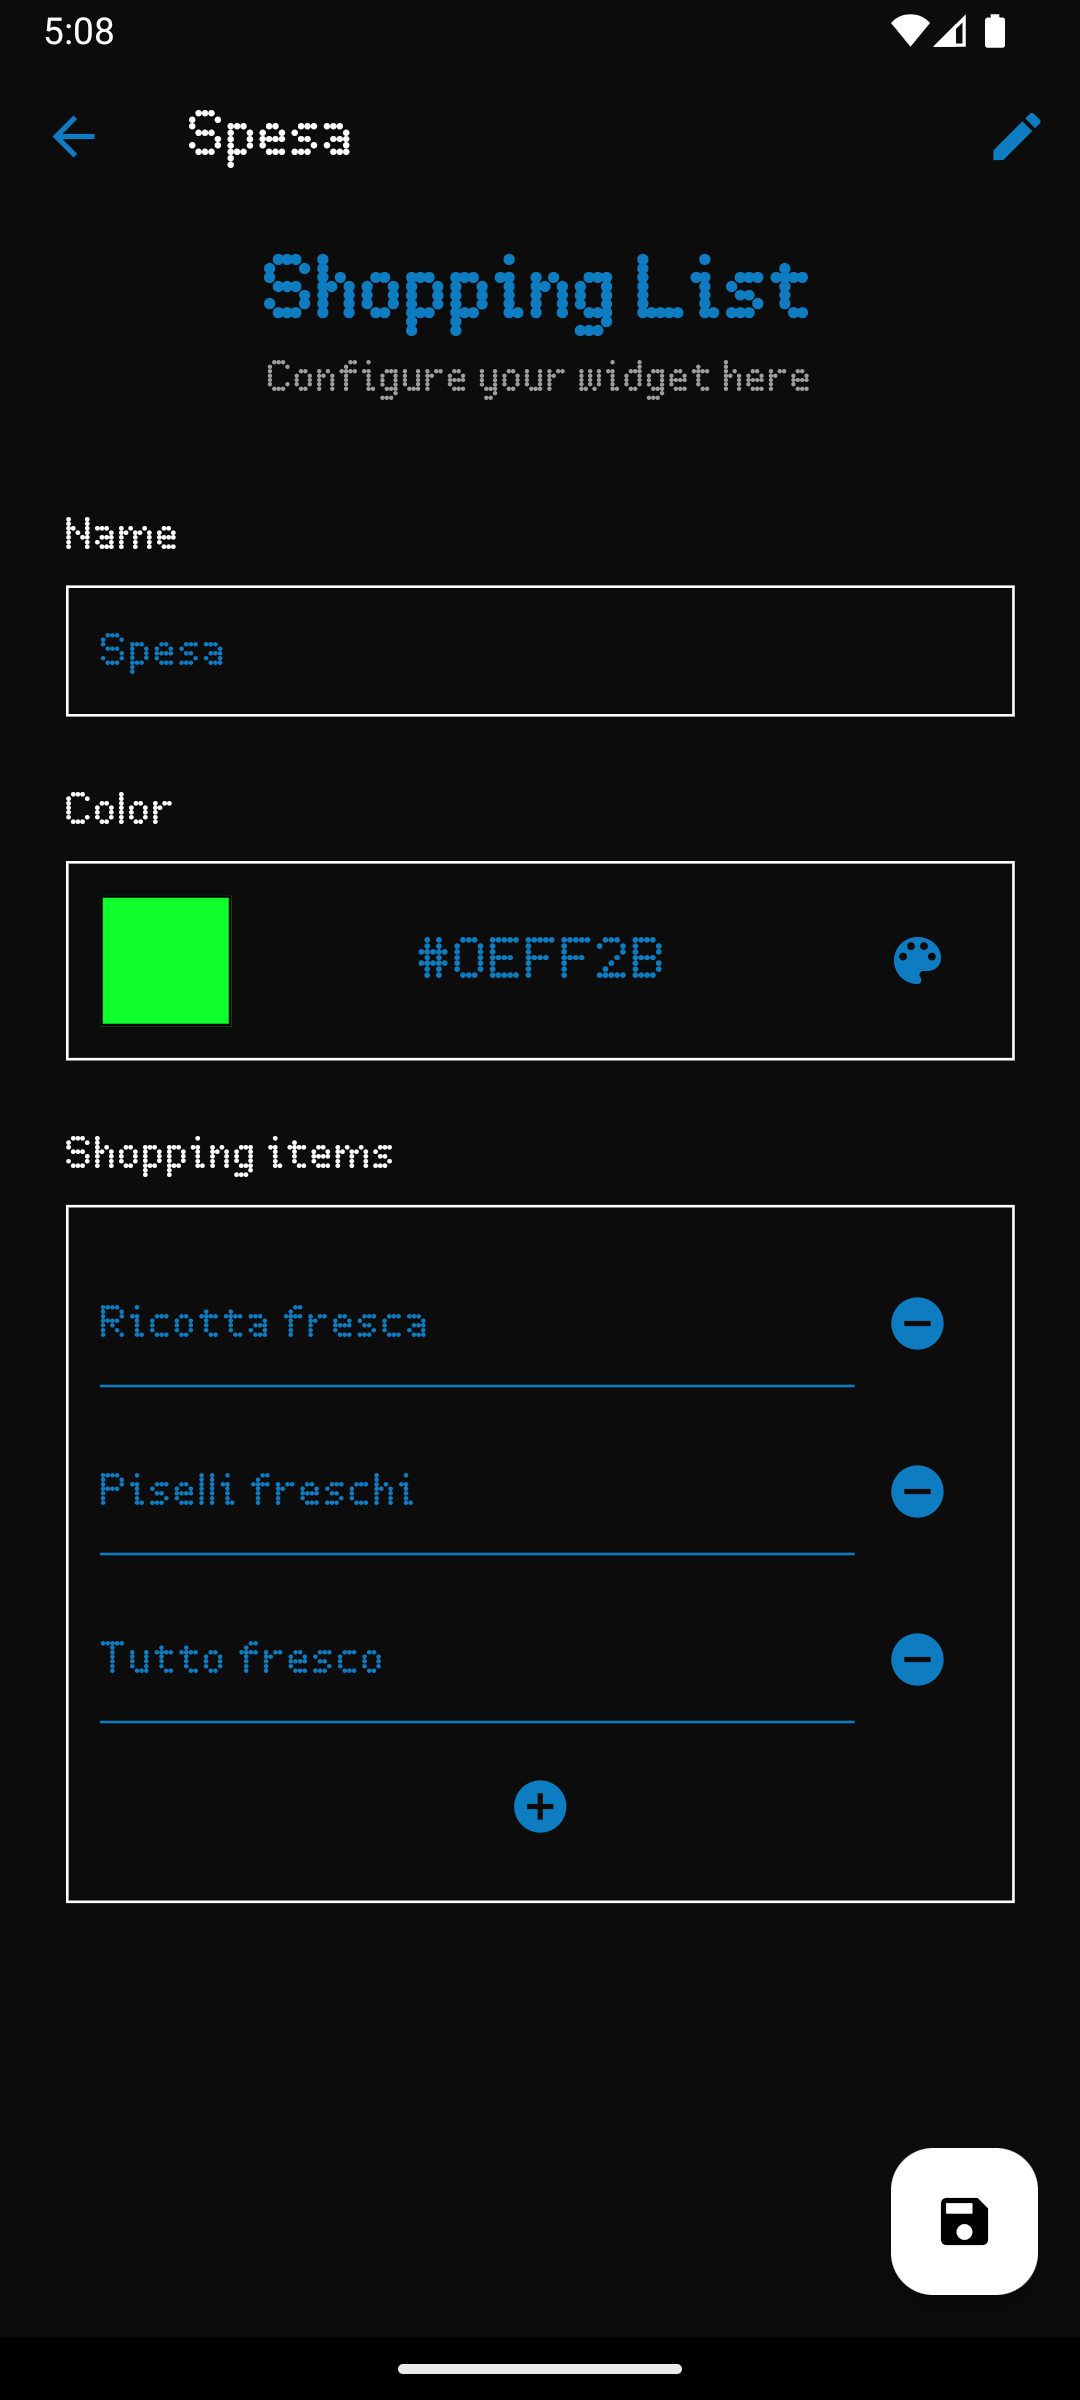
\includegraphics[width=\textwidth]{tesi/img/config_form/shopping_list_form.png}
\captionof{figure}{Client rendered form}
\end{minipage}

\subsection{Result of the Configuration}
The data collected from the user through the configuration form is saved in a JSON file. 
This file is parsed by the C++ engine when the specific widget with that configuration is loaded. 
Accessing the data from the configuration is straightforward in Python, as illustrated by the following example:

\begin{minipage}{0.65\textwidth}
\begin{minted}{python}
# config contains all the data from the configuration
from mosaico import widget, config

# Create title
text = widget.createText()
text.setText(config["name"])
text.setHexColor(config["color"])
text.moveTo(2,0)
text.setFont("9x18")

# Create items
items = []
bullets = []
for i in range(0, len(config["items"])):
    # Create bullet
    bullets.append(widget.createRectangle())
    bullets[i].setSize(2,2)        
    bullets[i].moveTo(4,16)
    bullets[i].translateYBy((i*7) + 5)    
    bullets[i].setHexColor(config["color"])  
    
    # Create entry  
    items.append(widget.createText())
    items[i].setFont("4x6")
    items[i].setText(config["items"][i])
    items[i].moveTo(8,14)    
    items[i].translateYBy((i*7) + 5)

def loop():
    pass
\end{minted}
\end{minipage}
\begin{minipage}{0.30\textwidth}
\centering
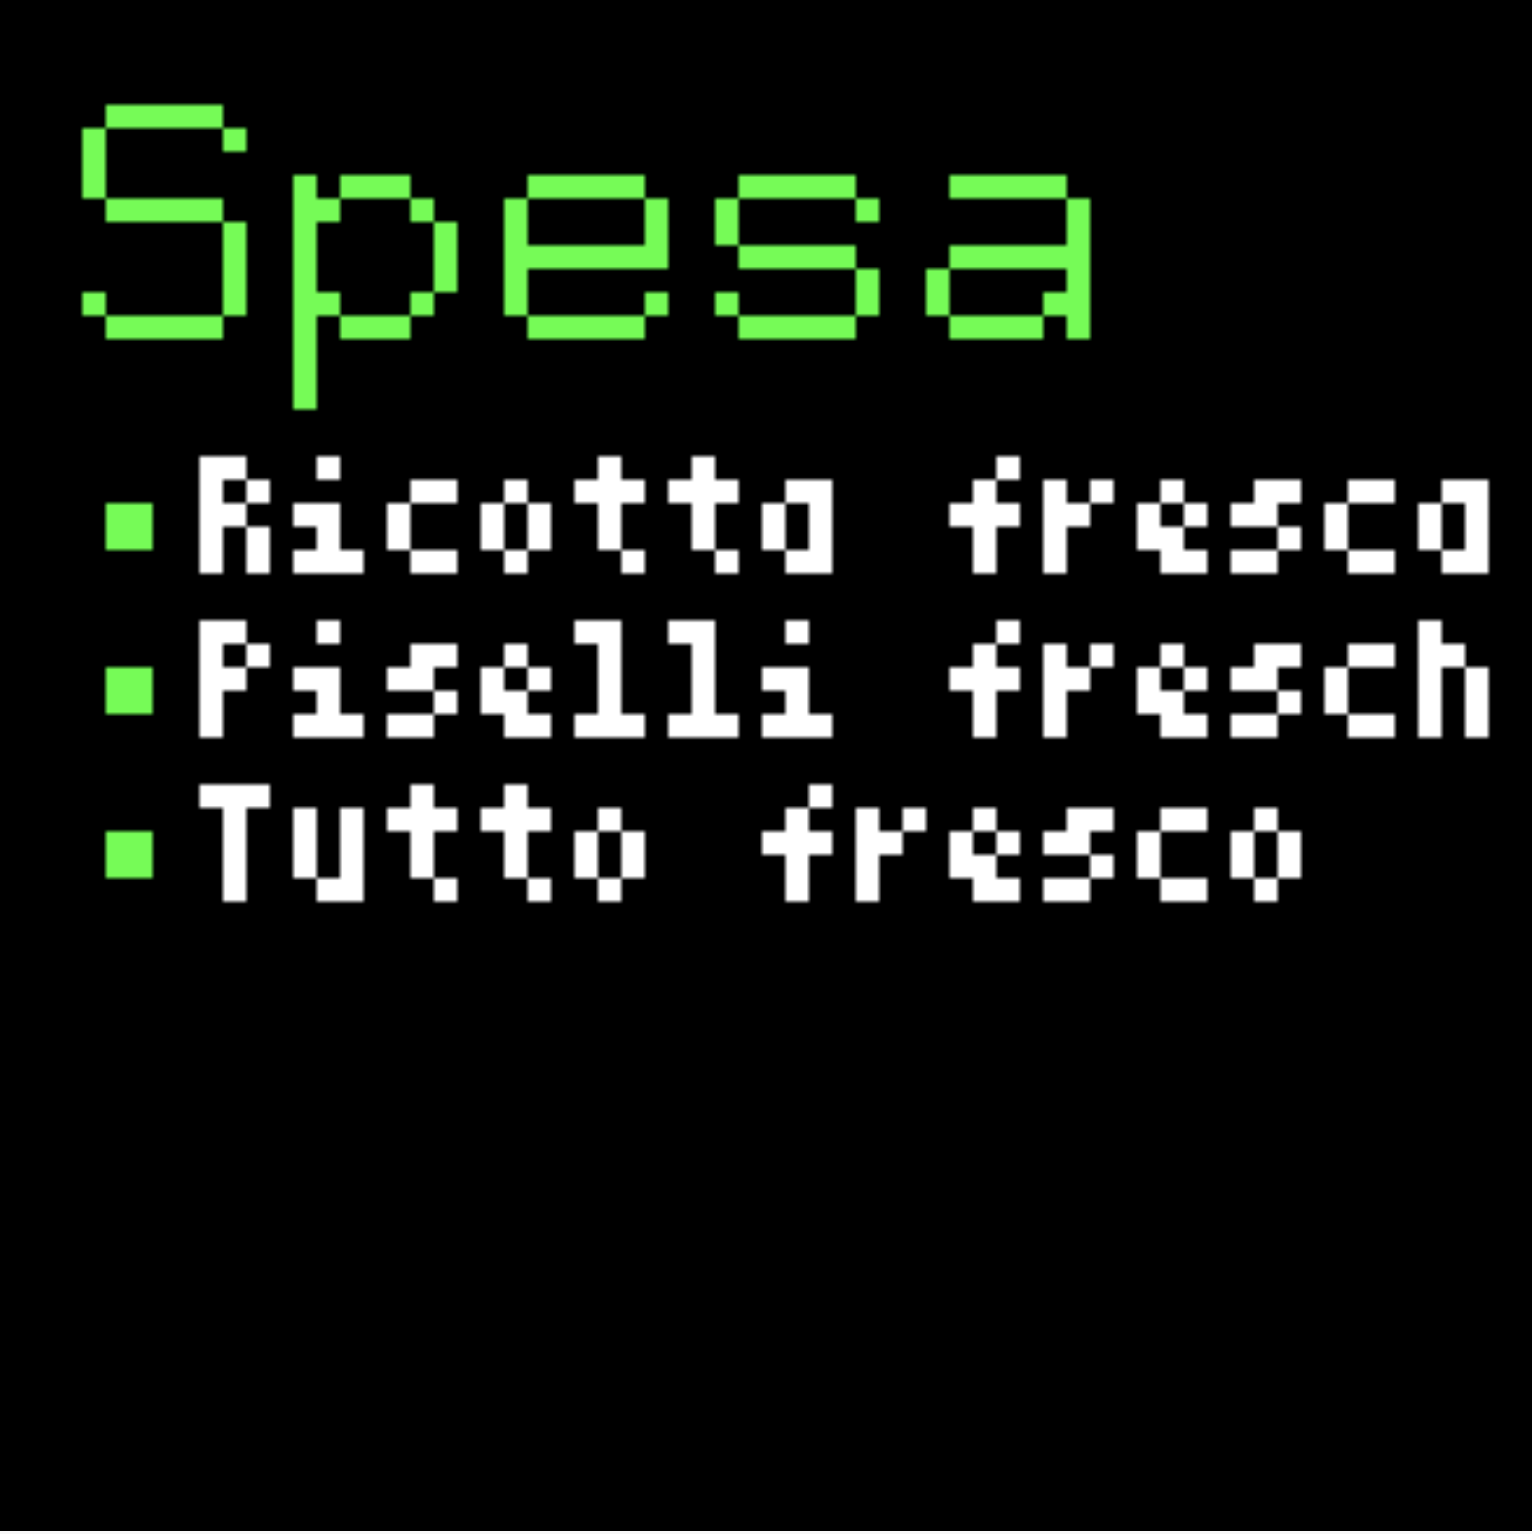
\includegraphics[width=\textwidth]{tesi/img/config_form/shopping_list_result.png}
\captionof{figure}{Result on matrix}
\end{minipage}

\subsection{Assets Management}
Each widget configuration is stored as a \texttt{.tar.gz} archive, which is essentially a compressed file that contains all the data submitted by the user. This compression facilitates faster transfers. Inside the archive, there is a \texttt{.json} file that holds the configuration details, as well as any additional binary files (e.g., images or other assets) uploaded by the user. A helper function is available to easily retrieve the path to these assets within the archive, simplifying access to the resources when needed.

\subsection{Field Attributes}
All fields share the following common attributes, regardless of their type:

\begin{itemize}
    \item \textbf{Name (required):} The unique identifier for the field within the configuration file. \textbf{Note:} \textit{You cannot use the same name for different fields}

    \item \textbf{Type (required):} Specifies the data type of the field. The type can be one of the following:
    \begin{itemize}
        \item \texttt{string}: A simple text field.
        \item \texttt{string[]}: An array of strings.
        \item \texttt{color}: A color picker field.
        \item \texttt{image}: An image upload field.
            \textbf{Special Attributes:}
            \begin{itemize}
            \item \texttt{Dimensions}: Specifies the image dimensions, as an object containing:
            \begin{itemize}
                \item \texttt{width}: The image width in pixels.
                \item \texttt{height}: The image height in pixels.
            \end{itemize}
            \end{itemize}
        \item \texttt{select}: An font selector between one of the available.
        \textbf{Special Attributes:}
            \begin{itemize}
            \item \texttt{options}: An array of strings, one will be selected by the user
            \end{itemize}
        \item \texttt{font}: An font selector between one of the available.
    \end{itemize}

    \item \textbf{Label:} The label displayed to the user in the configuration form to help them understand the purpose of the field.

    \item \textbf{Required:} A boolean value that indicates whether the field is mandatory.

    \item \textbf{Placeholder:} A placeholder text shown when the field is empty, providing guidance to the user about what to enter.
\end{itemize}


\subsection{Multiple configurations}
Obviously it would not make sense to create a configuration for one use only, once a configuration for a specific widget is created and user gave it a name, it will always be possible for them to list all the created, delete them or edit them using the appropriate 